\chapter{Corner Simulation}
Corner simulations are performed to verify that the circuit works at all possible conditions of process, supply voltage and temperature. Analog circuit designs that perform sufficiently well across these corners are to be considered a robust design.

\section{Process Variation}

Process variation is the naturally occurring variation in the attributes of transistors (length, widths, oxide thickness) when ICs are fabricated. In general there are 5 corners - tt, ff, ss, fs, sf. Transistors can be typical, fast or slow. The first letter indicates the PMOS and the second letter indicates the NMOS. However, as part of XT018 technology, the corners are termed as - tm, wp, ws, wo, wz. The meaning and their translation to the general conventions are described in Table.\ref{tab:Process_Corners}. The process corners of Capacitors and Resistors too follow a similar naming convention but with only 3 corners - tm (typical), wp(minimum), ws(maximum).

\begin{table} [H]
\centering
\begin{tabular}{@{}ccc@{}}
\toprule
Corner	& Expansion						& Translation	\\ \midrule
tm		& Typical Mean Condition 		& tt			\\
wp		& Worst Case Power Condition	& ff			\\
ws		& Worst Case Speed Condition 	& ss			\\
wo		& Worst Case One Condition 		& fs			\\
wz		& Worst Case Zero Condition 	& sf			\\
\bottomrule
\end{tabular}
\caption{Different Corners for MOS Transistors in XT018 Technology}
\label{tab:Process_Corners}
\end{table}

A total of 45 corners are simulated for 3 different values of $V_{bias}$ - 150mV, 400mV and 700mV. And the results are provided in the subsequent sections.

\subsubsection{Lowest $V_{bias}$}

\begin{figure} [H]
\centering
\includegraphics[scale=1]{Figures/Corners/Overall/Proc_Min/PDFs/Proc_Min_gain.pdf}
\caption{Histogram of System Gain due to Process Variation at $V_{bias}$=150mV}
\end{figure}

\begin{figure} [H]
\centering
\includegraphics[scale=1]{Figures/Corners/Overall/Proc_Min/PDFs/Proc_Min_bw.pdf}
\caption{Histogram of System Bandwidth due to Process Variation at $V_{bias}$=150mV}
\end{figure}

\begin{figure} [H]
\centering
\includegraphics[scale=1]{Figures/Corners/Overall/Proc_Min/PDFs/Proc_Min_imax.pdf}
\caption{Histogram of Maximum Output Current due to Process Variation at $V_{bias}$=150mV}
\end{figure}

\begin{figure} [H]
\centering
\includegraphics[scale=1]{Figures/Corners/Overall/Proc_Min/PDFs/Proc_Min_imin.pdf}
\caption{Histogram of Minimum Output Current due to Process Variation at $V_{bias}$=150mV}
\end{figure}

\begin{figure} [H]
\centering
\includegraphics[scale=1]{Figures/Corners/Overall/Proc_Min/PDFs/Proc_Min_gm.pdf}
\caption{Histogram of Transconductance due to Process Variation at $V_{bias}$=150mV}
\end{figure}

\begin{figure} [H]
\centering
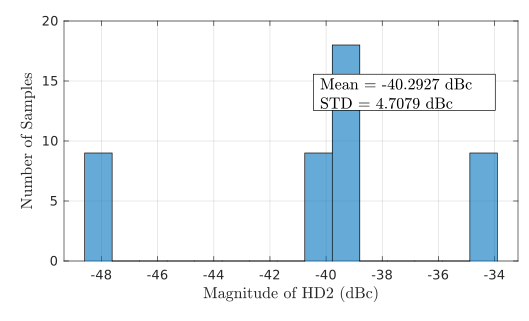
\includegraphics[scale=1]{Figures/Corners/Overall/Proc_Min/PDFs/Proc_Min_hd2.pdf}
\caption{Histogram of HD2 due to Process Variation at $V_{bias}$=150mV}
\end{figure}

\begin{figure} [H]
\centering
\includegraphics[scale=1]{Figures/Corners/Overall/Proc_Min/PDFs/Proc_Min_hd3.pdf}
\caption{Histogram of HD3 due to Process Variation at $V_{bias}$=150mV}
\end{figure}

\begin{figure} [H]
\centering
\includegraphics[scale=1]{Figures/Corners/Overall/Proc_Min/PDFs/Proc_Min_irn.pdf}
\caption{Histogram of Input Referred Noise due to Process Variation at $V_{bias}$=150mV}
\end{figure}

\begin{figure} [H]
\centering
\includegraphics[scale=1]{Figures/Corners/Overall/Proc_Min/PDFs/Proc_Min_zin.pdf}
\caption{Histogram of Input Impedance due to Process Variation at $V_{bias}$=150mV}
\end{figure}

\begin{figure} [H]
\centering
\includegraphics[scale=1]{Figures/Corners/Overall/Proc_Min/PDFs/Proc_Min_zout.pdf}
\caption{Histogram of Output Impedance due to Process Variation at $V_{bias}$=150mV}
\end{figure}

\begin{figure} [H]
\centering
\includegraphics[scale=1]{Figures/Corners/Overall/Proc_Min/PDFs/Proc_Min_psrrp.pdf}
\caption{Histogram of PSRR($V_{DD}$) due to Process Variation at $V_{bias}$=150mV}
\end{figure}

\begin{figure} [H]
\centering
\includegraphics[scale=1]{Figures/Corners/Overall/Proc_Min/PDFs/Proc_Min_psrrn.pdf}
\caption{Histogram of PSRR($V_{SS}$) due to Process Variation at $V_{bias}$=150mV}
\end{figure}

\subsubsection{Middle $V_{bias}$}

\begin{figure} [H]
\centering
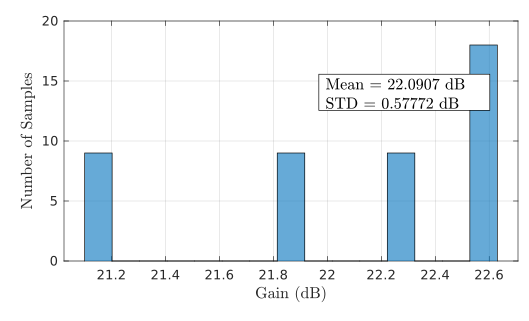
\includegraphics[scale=1]{Figures/Corners/Overall/Proc_Mid/PDFs/Proc_Mid_gain.pdf}
\caption{Histogram of System Gain due to Process Variation at $V_{bias}$=400mV}
\end{figure}

\begin{figure} [H]
\centering
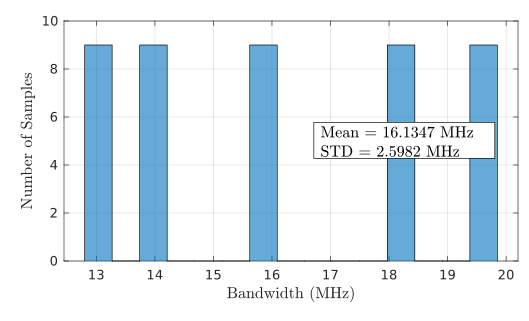
\includegraphics[scale=1]{Figures/Corners/Overall/Proc_Mid/PDFs/Proc_Mid_bw.pdf}
\caption{Histogram of System Bandwidth due to Process Variation at $V_{bias}$=400mV}
\end{figure}

\begin{figure} [H]
\centering
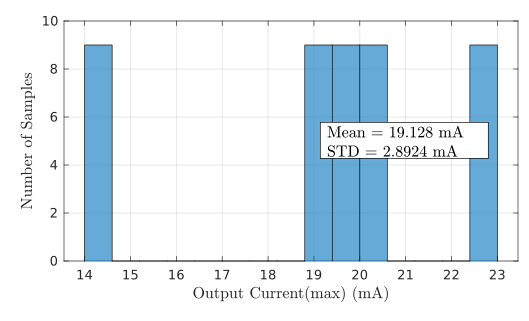
\includegraphics[scale=1]{Figures/Corners/Overall/Proc_Mid/PDFs/Proc_Mid_imax.pdf}
\caption{Histogram of Maximum Output Current due to Process Variation at $V_{bias}$=400mV}
\end{figure}

\begin{figure} [H]
\centering
\includegraphics[scale=1]{Figures/Corners/Overall/Proc_Mid/PDFs/Proc_Mid_imin.pdf}
\caption{Histogram of Minimum Output Current due to Process Variation at $V_{bias}$=400mV}
\end{figure}

\begin{figure} [H]
\centering
\includegraphics[scale=1]{Figures/Corners/Overall/Proc_Mid/PDFs/Proc_Mid_gm.pdf}
\caption{Histogram of Transconductance due to Process Variation at $V_{bias}$=400mV}
\end{figure}

\begin{figure} [H]
\centering
\includegraphics[scale=1]{Figures/Corners/Overall/Proc_Mid/PDFs/Proc_Mid_hd2.pdf}
\caption{Histogram of HD2 due to Process Variation at $V_{bias}$=400mV}
\end{figure}

\begin{figure} [H]
\centering
\includegraphics[scale=1]{Figures/Corners/Overall/Proc_Mid/PDFs/Proc_Mid_hd3.pdf}
\caption{Histogram of HD3 due to Process Variation at $V_{bias}$=400mV}
\end{figure}

\begin{figure} [H]
\centering
\includegraphics[scale=1]{Figures/Corners/Overall/Proc_Mid/PDFs/Proc_Mid_irn.pdf}
\caption{Histogram of Input Referred Noise due to Process Variation at $V_{bias}$=400mV}
\end{figure}

\begin{figure} [H]
\centering
\includegraphics[scale=1]{Figures/Corners/Overall/Proc_Mid/PDFs/Proc_Mid_zin.pdf}
\caption{Histogram of Input Impedance due to Process Variation at $V_{bias}$=400mV}
\end{figure}

\begin{figure} [H]
\centering
\includegraphics[scale=1]{Figures/Corners/Overall/Proc_Mid/PDFs/Proc_Mid_zout.pdf}
\caption{Histogram of Output Impedance due to Process Variation at $V_{bias}$=400mV}
\end{figure}

\begin{figure} [H]
\centering
\includegraphics[scale=1]{Figures/Corners/Overall/Proc_Mid/PDFs/Proc_Mid_psrrp.pdf}
\caption{Histogram of PSRR($V_{DD}$) due to Process Variation at $V_{bias}$=400mV}
\end{figure}

\begin{figure} [H]
\centering
\includegraphics[scale=1]{Figures/Corners/Overall/Proc_Mid/PDFs/Proc_Mid_psrrn.pdf}
\caption{Histogram of PSRR($V_{SS}$) due to Process Variation at $V_{bias}$=400mV}
\end{figure}

\subsubsection{Highest $V_{bias}$}

\begin{figure} [H]
\centering
\includegraphics[scale=1]{Figures/Corners/Overall/Proc_Max/PDFs/Proc_Max_gain.pdf}
\caption{Histogram of System Gain due to Process Variation at $V_{bias}$=700mV}
\end{figure}

\begin{figure} [H]
\centering
\includegraphics[scale=1]{Figures/Corners/Overall/Proc_Max/PDFs/Proc_Max_bw.pdf}
\caption{Histogram of System Bandwidth due to Process Variation at $V_{bias}$=700mV}
\end{figure}

\begin{figure} [H]
\centering
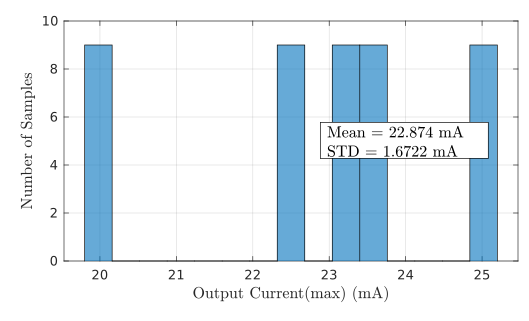
\includegraphics[scale=1]{Figures/Corners/Overall/Proc_Max/PDFs/Proc_Max_imax.pdf}
\caption{Histogram of Maximum Output Current due to Process Variation at $V_{bias}$=700mV}
\end{figure}

\begin{figure} [H]
\centering
\includegraphics[scale=1]{Figures/Corners/Overall/Proc_Max/PDFs/Proc_Max_imin.pdf}
\caption{Histogram of Minimum Output Current due to Process Variation at $V_{bias}$=700mV}
\end{figure}

\begin{figure} [H]
\centering
\includegraphics[scale=1]{Figures/Corners/Overall/Proc_Max/PDFs/Proc_Max_gm.pdf}
\caption{Histogram of Transconductance due to Process Variation at $V_{bias}$=700mV}
\end{figure}

\begin{figure} [H]
\centering
\includegraphics[scale=1]{Figures/Corners/Overall/Proc_Max/PDFs/Proc_Max_hd2.pdf}
\caption{Histogram of HD2 due to Process Variation at $V_{bias}$=700mV}
\end{figure}

\begin{figure} [H]
\centering
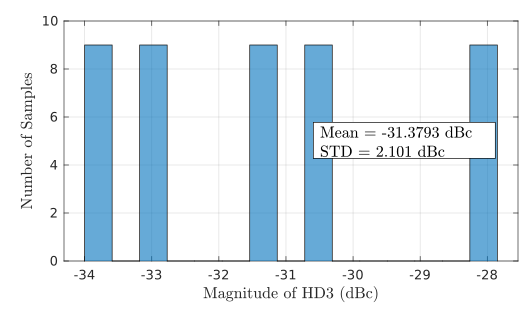
\includegraphics[scale=1]{Figures/Corners/Overall/Proc_Max/PDFs/Proc_Max_hd3.pdf}
\caption{Histogram of HD3 due to Process Variation at $V_{bias}$=700mV}
\end{figure}

\begin{figure} [H]
\centering
\includegraphics[scale=1]{Figures/Corners/Overall/Proc_Max/PDFs/Proc_Max_irn.pdf}
\caption{Histogram of Input Referred Noise due to Process Variation at $V_{bias}$=400mV}
\end{figure}

\begin{figure} [H]
\centering
\includegraphics[scale=1]{Figures/Corners/Overall/Proc_Max/PDFs/Proc_Max_zin.pdf}
\caption{Histogram of Input Impedance due to Process Variation at $V_{bias}$=700mV}
\end{figure}

\begin{figure} [H]
\centering
\includegraphics[scale=1]{Figures/Corners/Overall/Proc_Max/PDFs/Proc_Max_zout.pdf}
\caption{Histogram of Output Impedance due to Process Variation at $V_{bias}$=700mV}
\end{figure}

\begin{figure} [H]
\centering
\includegraphics[scale=1]{Figures/Corners/Overall/Proc_Max/PDFs/Proc_Max_psrrp.pdf}
\caption{Histogram of PSRR($V_{DD}$) due to Process Variation at $V_{bias}$=700mV}
\end{figure}

\begin{figure} [H]
\centering
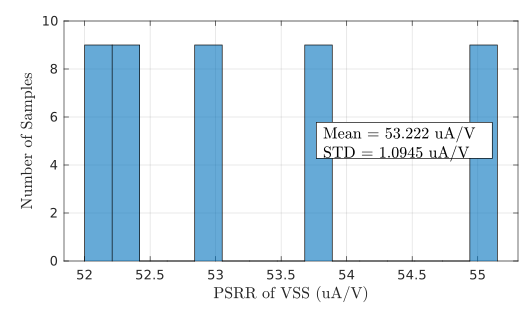
\includegraphics[scale=1]{Figures/Corners/Overall/Proc_Max/PDFs/Proc_Max_psrrn.pdf}
\caption{Histogram of PSRR($V_{SS}$) due to Process Variation at $V_{bias}$=700mV}
\end{figure}

\section{Process and Supply Variation}

In addition to process variation, the system responds to power supply variations too. 3 different corners are obtained by evaluating the power supply with $\pm$10\% from the nominal value. Therefore, we get 3 corners for $V_{DD}$ - 2.5V, 2.25V, 2.75V and 3 corners for $V_{SS}$ - -2.5V, -2.25V, -2.75V. The total number of corners in this case are 405. And the results are discussed in the subsequent sections.

\subsubsection{Lowest $V_{bias}$}

\begin{figure} [H]
\centering
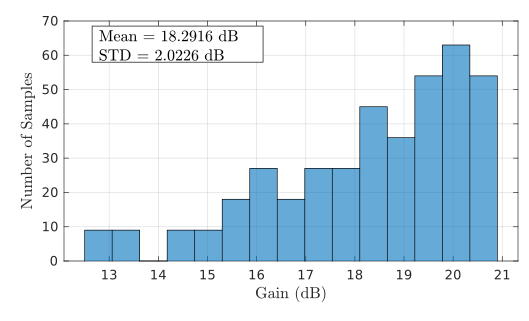
\includegraphics[scale=1]{Figures/Corners/Overall/PV_Min/PDFs/PV_Min_gain.pdf}
\caption{Histogram of System Gain due to Process and Supply Variation at $V_{bias}$=150mV}
\end{figure}

\begin{figure} [H]
\centering
\includegraphics[scale=1]{Figures/Corners/Overall/PV_Min/PDFs/PV_Min_bw.pdf}
\caption{Histogram of System Bandwidth due to Process and Supply Variation at $V_{bias}$=150mV}
\end{figure}

\begin{figure} [H]
\centering
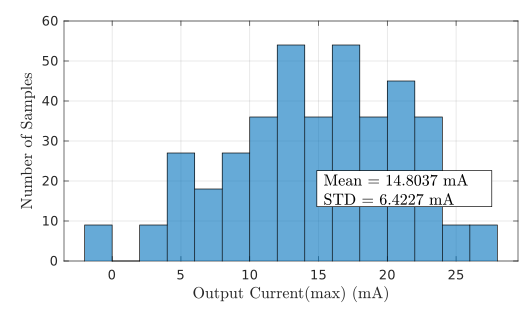
\includegraphics[scale=1]{Figures/Corners/Overall/PV_Min/PDFs/PV_Min_imax.pdf}
\caption{Histogram of Maximum Output Current due to Process and Supply Variation at $V_{bias}$=150mV}
\end{figure}

\begin{figure} [H]
\centering
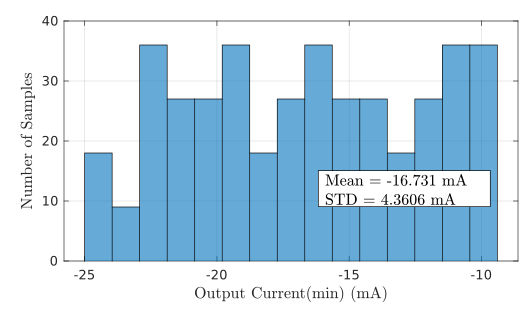
\includegraphics[scale=1]{Figures/Corners/Overall/PV_Min/PDFs/PV_Min_imin.pdf}
\caption{Histogram of Minimum Output Current due to Process and Supply Variation at $V_{bias}$=150mV}
\end{figure}

\begin{figure} [H]
\centering
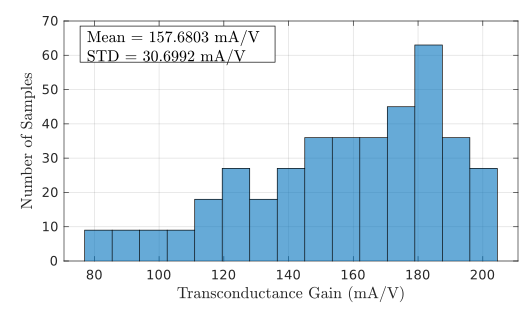
\includegraphics[scale=1]{Figures/Corners/Overall/PV_Min/PDFs/PV_Min_gm.pdf}
\caption{Histogram of Transconductance due to Process and Supply Variation at $V_{bias}$=150mV}
\end{figure}

\begin{figure} [H]
\centering
\includegraphics[scale=1]{Figures/Corners/Overall/PV_Min/PDFs/PV_Min_hd2.pdf}
\caption{Histogram of HD2 due to Process and Supply Variation at $V_{bias}$=150mV}
\end{figure}

\begin{figure} [H]
\centering
\includegraphics[scale=1]{Figures/Corners/Overall/PV_Min/PDFs/PV_Min_hd3.pdf}
\caption{Histogram of HD3 due to Process and Supply Variation at $V_{bias}$=150mV}
\end{figure}

\begin{figure} [H]
\centering
\includegraphics[scale=1]{Figures/Corners/Overall/PV_Min/PDFs/PV_Min_irn.pdf}
\caption{Histogram of Input Referred Noise due to Process and Supply Variation at $V_{bias}$=150mV}
\end{figure}

\begin{figure} [H]
\centering
\includegraphics[scale=1]{Figures/Corners/Overall/PV_Min/PDFs/PV_Min_zin.pdf}
\caption{Histogram of Input Impedance due to Process and Supply Variation at $V_{bias}$=150mV}
\end{figure}

\begin{figure} [H]
\centering
\includegraphics[scale=1]{Figures/Corners/Overall/PV_Min/PDFs/PV_Min_zout.pdf}
\caption{Histogram of Output Impedance due to Process and Supply Variation at $V_{bias}$=150mV}
\end{figure}

\begin{figure} [H]
\centering
\includegraphics[scale=1]{Figures/Corners/Overall/PV_Min/PDFs/PV_Min_psrrp.pdf}
\caption{Histogram of PSRR($V_{DD}$) due to Process and SUpply Variation at $V_{bias}$=150mV}
\end{figure}

\begin{figure} [H]
\centering
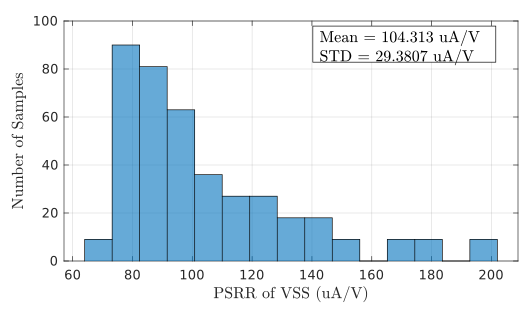
\includegraphics[scale=1]{Figures/Corners/Overall/PV_Min/PDFs/PV_Min_psrrn.pdf}
\caption{Histogram of PSRR($V_{SS}$) due to Process and SUpply Variation at $V_{bias}$=150mV}
\end{figure}

\subsubsection{Middle $V_{bias}$}

\begin{figure} [H]
\centering
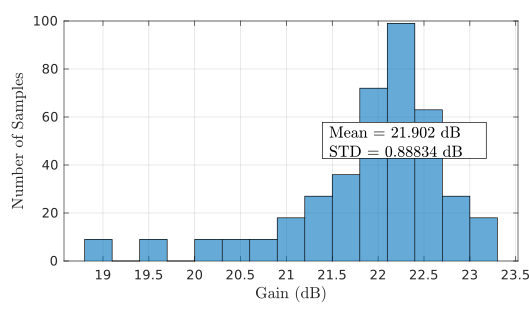
\includegraphics[scale=1]{Figures/Corners/Overall/PV_Mid/PDFs/PV_Mid_gain.pdf}
\caption{Histogram of System Gain due to Process and Supply Variation at $V_{bias}$=400mV}
\end{figure}

\begin{figure} [H]
\centering
\includegraphics[scale=1]{Figures/Corners/Overall/PV_Mid/PDFs/PV_Mid_bw.pdf}
\caption{Histogram of System Bandwidth due to Process and Supply Variation at $V_{bias}$=400mV}
\end{figure}

\begin{figure} [H]
\centering
\includegraphics[scale=1]{Figures/Corners/Overall/PV_Mid/PDFs/PV_Mid_imax.pdf}
\caption{Histogram of Maximum Output Current due to Process and Supply Variation at $V_{bias}$=400mV}
\end{figure}

\begin{figure} [H]
\centering
\includegraphics[scale=1]{Figures/Corners/Overall/PV_Mid/PDFs/PV_Mid_imin.pdf}
\caption{Histogram of Minimum Output Current due to Process and Supply Variation at $V_{bias}$=400mV}
\end{figure}

\begin{figure} [H]
\centering
\includegraphics[scale=1]{Figures/Corners/Overall/PV_Mid/PDFs/PV_Mid_gm.pdf}
\caption{Histogram of Transconductance due to Process and Supply Variation at $V_{bias}$=400mV}
\end{figure}

\begin{figure} [H]
\centering
\includegraphics[scale=1]{Figures/Corners/Overall/PV_Mid/PDFs/PV_Mid_hd2.pdf}
\caption{Histogram of HD2 due to Process and Supply Variation at $V_{bias}$=400mV}
\end{figure}

\begin{figure} [H]
\centering
\includegraphics[scale=1]{Figures/Corners/Overall/PV_Mid/PDFs/PV_Mid_hd3.pdf}
\caption{Histogram of HD3 due to Process and Supply Variation at $V_{bias}$=400mV}
\end{figure}

\begin{figure} [H]
\centering
\includegraphics[scale=1]{Figures/Corners/Overall/PV_Mid/PDFs/PV_Mid_irn.pdf}
\caption{Histogram of Input Referred Noise due to Process and Supply Variation at $V_{bias}$=400mV}
\end{figure}

\begin{figure} [H]
\centering
\includegraphics[scale=1]{Figures/Corners/Overall/PV_Mid/PDFs/PV_Mid_zin.pdf}
\caption{Histogram of Input Impedance due to Process and Supply Variation at $V_{bias}$=400mV}
\end{figure}

\begin{figure} [H]
\centering
\includegraphics[scale=1]{Figures/Corners/Overall/PV_Mid/PDFs/PV_Mid_zout.pdf}
\caption{Histogram of Output Impedance due to Process and Supply Variation at $V_{bias}$=400mV}
\end{figure}

\begin{figure} [H]
\centering
\includegraphics[scale=1]{Figures/Corners/Overall/PV_Mid/PDFs/PV_Mid_psrrp.pdf}
\caption{Histogram of PSRR($V_{DD}$) due to Process and Supply Variation at $V_{bias}$=400mV}
\end{figure}

\begin{figure} [H]
\centering
\includegraphics[scale=1]{Figures/Corners/Overall/PV_Mid/PDFs/PV_Mid_psrrn.pdf}
\caption{Histogram of PSRR($V_{SS}$) due to Process and Supply Variation at $V_{bias}$=400mV}
\end{figure}

\subsubsection{Highest $V_{bias}$}

\begin{figure} [H]
\centering
\includegraphics[scale=1]{Figures/Corners/Overall/PV_Max/PDFs/PV_Max_gain.pdf}
\caption{Histogram of System Gain due to Process and Supply Variation at $V_{bias}$=700mV}
\end{figure}

\begin{figure} [H]
\centering
\includegraphics[scale=1]{Figures/Corners/Overall/PV_Max/PDFs/PV_Max_bw.pdf}
\caption{Histogram of System Bandwidth due to Process and Supply Variation at $V_{bias}$=700mV}
\end{figure}

\begin{figure} [H]
\centering
\includegraphics[scale=1]{Figures/Corners/Overall/PV_Max/PDFs/PV_Max_imax.pdf}
\caption{Histogram of Maximum Output Current due to Process and Supply Variation at $V_{bias}$=700mV}
\end{figure}

\begin{figure} [H]
\centering
\includegraphics[scale=1]{Figures/Corners/Overall/PV_Max/PDFs/PV_Max_imin.pdf}
\caption{Histogram of Minimum Output Current due to Process and Supply Variation at $V_{bias}$=700mV}
\end{figure}

\begin{figure} [H]
\centering
\includegraphics[scale=1]{Figures/Corners/Overall/PV_Max/PDFs/PV_Max_gm.pdf}
\caption{Histogram of Transconductance due to Process and Supply Variation at $V_{bias}$=700mV}
\end{figure}

\begin{figure} [H]
\centering
\includegraphics[scale=1]{Figures/Corners/Overall/PV_Max/PDFs/PV_Max_hd2.pdf}
\caption{Histogram of HD2 due to Process and Supply Variation at $V_{bias}$=700mV}
\end{figure}

\begin{figure} [H]
\centering
\includegraphics[scale=1]{Figures/Corners/Overall/PV_Max/PDFs/PV_Max_hd3.pdf}
\caption{Histogram of HD3 due to Process and Supply Variation at $V_{bias}$=700mV}
\end{figure}

\begin{figure} [H]
\centering
\includegraphics[scale=1]{Figures/Corners/Overall/PV_Max/PDFs/PV_Max_irn.pdf}
\caption{Histogram of Input Referred Noise due to Process and Supply Variation at $V_{bias}$=400mV}
\end{figure}

\begin{figure} [H]
\centering
\includegraphics[scale=1]{Figures/Corners/Overall/PV_Max/PDFs/PV_Max_zin.pdf}
\caption{Histogram of Input Impedance due to Process and Supply Variation at $V_{bias}$=700mV}
\end{figure}

\begin{figure} [H]
\centering
\includegraphics[scale=1]{Figures/Corners/Overall/PV_Max/PDFs/PV_Max_zout.pdf}
\caption{Histogram of Output Impedance due to Process and Supply Variation at $V_{bias}$=700mV}
\end{figure}

\begin{figure} [H]
\centering
\includegraphics[scale=1]{Figures/Corners/Overall/PV_Max/PDFs/PV_Max_psrrp.pdf}
\caption{Histogram of PSRR($V_{DD}$) due to Process and Supply Variation at $V_{bias}$=700mV}
\end{figure}

\begin{figure} [H]
\centering
\includegraphics[scale=1]{Figures/Corners/Overall/PV_Max/PDFs/PV_Max_psrrn.pdf}
\caption{Histogram of PSRR($V_{SS}$) due to Process and Supply Variation at $V_{bias}$=700mV}
\end{figure}
 
\section{Process, Voltage and Temperature (PVT) variation}

Another possible variation is seen in the temperature parameter. The PVT corner simulations are performed at the following corners:
\begin{itemize}
\item All Process corners mentioned in Section 4.6.1.
\item $\pm$10\% variations of $V_{DD}$ i.e., 2.5V, 2.25V, 2.75V and $V_{SS}$ i.e., -2.5V, -2.25V, -2.75V.
\item Three temperature conditions: -25$^0$C, 25$^0$C and 80$^0$C.
\end{itemize}

Therefore, there are 1215 corners in total. The results are provided in the subsequent sections.

\subsubsection{Lowest $V_{bias}$}

\begin{figure} [H]
\centering
\includegraphics[scale=1]{Figures/Corners/Overall/PVT_Min/PDFs/PVT_Min_gain.pdf}
\caption{Histogram of System Gain due to PVT Variation at $V_{bias}$=150mV}
\end{figure}

\begin{figure} [H]
\centering
\includegraphics[scale=1]{Figures/Corners/Overall/PVT_Min/PDFs/PVT_Min_bw.pdf}
\caption{Histogram of System Bandwidth due to PVT Variation at $V_{bias}$=150mV}
\end{figure}

\begin{figure} [H]
\centering
\includegraphics[scale=1]{Figures/Corners/Overall/PVT_Min/PDFs/PVT_Min_imax.pdf}
\caption{Histogram of Maximum Output Current due to PVT Variation at $V_{bias}$=150mV}
\end{figure}

\begin{figure} [H]
\centering
\includegraphics[scale=1]{Figures/Corners/Overall/PVT_Min/PDFs/PVT_Min_imin.pdf}
\caption{Histogram of Minimum Output Current due to PVT Variation at $V_{bias}$=150mV}
\end{figure}

\begin{figure} [H]
\centering
\includegraphics[scale=1]{Figures/Corners/Overall/PVT_Min/PDFs/PVT_Min_gm.pdf}
\caption{Histogram of Transconductance due to PVT Variation at $V_{bias}$=150mV}
\end{figure}

\begin{figure} [H]
\centering
\includegraphics[scale=1]{Figures/Corners/Overall/PVT_Min/PDFs/PVT_Min_hd2.pdf}
\caption{Histogram of HD2 due to PVT Variation at $V_{bias}$=150mV}
\end{figure}

\begin{figure} [H]
\centering
\includegraphics[scale=1]{Figures/Corners/Overall/PVT_Min/PDFs/PVT_Min_hd3.pdf}
\caption{Histogram of HD3 due to PVT at $V_{bias}$=150mV}
\end{figure}

\begin{figure} [H]
\centering
\includegraphics[scale=1]{Figures/Corners/Overall/PVT_Min/PDFs/PVT_Min_irn.pdf}
\caption{Histogram of Input Referred Noise due to PVT Variation at $V_{bias}$=150mV}
\end{figure}

\begin{figure} [H]
\centering
\includegraphics[scale=1]{Figures/Corners/Overall/PVT_Min/PDFs/PVT_Min_zin.pdf}
\caption{Histogram of Input Impedance due to PVT Variation at $V_{bias}$=150mV}
\end{figure}

\begin{figure} [H]
\centering
\includegraphics[scale=1]{Figures/Corners/Overall/PVT_Min/PDFs/PVT_Min_zout.pdf}
\caption{Histogram of Output Impedance due to PVT Variation at $V_{bias}$=150mV}
\end{figure}

\begin{figure} [H]
\centering
\includegraphics[scale=1]{Figures/Corners/Overall/PVT_Min/PDFs/PVT_Min_psrrp.pdf}
\caption{Histogram of PSRR($V_{DD}$) due to PVT Variation at $V_{bias}$=150mV}
\end{figure}

\begin{figure} [H]
\centering
\includegraphics[scale=1]{Figures/Corners/Overall/PVT_Min/PDFs/PVT_Min_psrrn.pdf}
\caption{Histogram of PSRR($V_{SS}$) due to PVT Variation at $V_{bias}$=150mV}
\end{figure}

\subsubsection{Middle $V_{bias}$}

\begin{figure} [H]
\centering
\includegraphics[scale=1]{Figures/Corners/Overall/PVT_Mid/PDFs/PVT_Mid_gain.pdf}
\caption{Histogram of System Gain due to PVT Variation at $V_{bias}$=400mV}
\end{figure}

\begin{figure} [H]
\centering
\includegraphics[scale=1]{Figures/Corners/Overall/PVT_Mid/PDFs/PVT_Mid_bw.pdf}
\caption{Histogram of System Bandwidth due to PVT Variation at $V_{bias}$=400mV}
\end{figure}

\begin{figure} [H]
\centering
\includegraphics[scale=1]{Figures/Corners/Overall/PVT_Mid/PDFs/PVT_Mid_imax.pdf}
\caption{Histogram of Maximum Output Current due to PVT Variation at $V_{bias}$=400mV}
\end{figure}

\begin{figure} [H]
\centering
\includegraphics[scale=1]{Figures/Corners/Overall/PVT_Mid/PDFs/PVT_Mid_imin.pdf}
\caption{Histogram of Minimum Output Current due to PVT Variation at $V_{bias}$=400mV}
\end{figure}

\begin{figure} [H]
\centering
\includegraphics[scale=1]{Figures/Corners/Overall/PVT_Mid/PDFs/PVT_Mid_gm.pdf}
\caption{Histogram of Transconductance due to PVT Variation at $V_{bias}$=400mV}
\end{figure}

\begin{figure} [H]
\centering
\includegraphics[scale=1]{Figures/Corners/Overall/PVT_Mid/PDFs/PVT_Mid_hd2.pdf}
\caption{Histogram of HD2 due to PVT Variation at $V_{bias}$=400mV}
\end{figure}

\begin{figure} [H]
\centering
\includegraphics[scale=1]{Figures/Corners/Overall/PVT_Mid/PDFs/PVT_Mid_hd3.pdf}
\caption{Histogram of HD3 due to PVT Variation at $V_{bias}$=400mV}
\end{figure}

\begin{figure} [H]
\centering
\includegraphics[scale=1]{Figures/Corners/Overall/PVT_Mid/PDFs/PVT_Mid_irn.pdf}
\caption{Histogram of Input Referred Noise due to PVT Variation at $V_{bias}$=400mV}
\end{figure}

\begin{figure} [H]
\centering
\includegraphics[scale=1]{Figures/Corners/Overall/PVT_Mid/PDFs/PVT_Mid_zin.pdf}
\caption{Histogram of Input Impedance due to PVT Variation at $V_{bias}$=400mV}
\end{figure}

\begin{figure} [H]
\centering
\includegraphics[scale=1]{Figures/Corners/Overall/PVT_Mid/PDFs/PVT_Mid_zout.pdf}
\caption{Histogram of Output Impedance due to PVT Variation at $V_{bias}$=400mV}
\end{figure}

\begin{figure} [H]
\centering
\includegraphics[scale=1]{Figures/Corners/Overall/PVT_Mid/PDFs/PVT_Mid_psrrp.pdf}
\caption{Histogram of PSRR($V_{DD}$) due to PVT Variation at $V_{bias}$=400mV}
\end{figure}

\begin{figure} [H]
\centering
\includegraphics[scale=1]{Figures/Corners/Overall/PVT_Mid/PDFs/PVT_Mid_psrrn.pdf}
\caption{Histogram of PSRR($V_{SS}$) due to PVT Variation at $V_{bias}$=400mV}
\end{figure}

\subsubsection{Highest $V_{bias}$}

\begin{figure} [H]
\centering
\includegraphics[scale=1]{Figures/Corners/Overall/PVT_Max/PDFs/PVT_Max_gain.pdf}
\caption{Histogram of System Gain due to PVT Variation at $V_{bias}$=700mV}
\end{figure}

\begin{figure} [H]
\centering
\includegraphics[scale=1]{Figures/Corners/Overall/PVT_Max/PDFs/PVT_Max_bw.pdf}
\caption{Histogram of System Bandwidth due to PVT Variation at $V_{bias}$=700mV}
\end{figure}

\begin{figure} [H]
\centering
\includegraphics[scale=1]{Figures/Corners/Overall/PVT_Max/PDFs/PVT_Max_imax.pdf}
\caption{Histogram of Maximum Output Current due to PVT Variation at $V_{bias}$=700mV}
\end{figure}

\begin{figure} [H]
\centering
\includegraphics[scale=1]{Figures/Corners/Overall/PVT_Max/PDFs/PVT_Max_imin.pdf}
\caption{Histogram of Minimum Output Current due to PVT Variation at $V_{bias}$=700mV}
\end{figure}

\begin{figure} [H]
\centering
\includegraphics[scale=1]{Figures/Corners/Overall/PVT_Max/PDFs/PVT_Max_gm.pdf}
\caption{Histogram of Transconductance due to PVT Variation at $V_{bias}$=700mV}
\end{figure}

\begin{figure} [H]
\centering
\includegraphics[scale=1]{Figures/Corners/Overall/PVT_Max/PDFs/PVT_Max_hd2.pdf}
\caption{Histogram of HD2 due to PVT Variation at $V_{bias}$=700mV}
\end{figure}

\begin{figure} [H]
\centering
\includegraphics[scale=1]{Figures/Corners/Overall/PVT_Max/PDFs/PVT_Max_hd3.pdf}
\caption{Histogram of HD3 due to PVT Variation at $V_{bias}$=700mV}
\end{figure}

\begin{figure} [H]
\centering
\includegraphics[scale=1]{Figures/Corners/Overall/PVT_Max/PDFs/PVT_Max_irn.pdf}
\caption{Histogram of Input Referred Noise due to PVT Variation at $V_{bias}$=400mV}
\end{figure}

\begin{figure} [H]
\centering
\includegraphics[scale=1]{Figures/Corners/Overall/PVT_Max/PDFs/PVT_Max_zin.pdf}
\caption{Histogram of Input Impedance due to PVT Variation at $V_{bias}$=700mV}
\end{figure}

\begin{figure} [H]
\centering
\includegraphics[scale=1]{Figures/Corners/Overall/PVT_Max/PDFs/PVT_Max_zout.pdf}
\caption{Histogram of Output Impedance due to Process and Supply Variation at $V_{bias}$=700mV}
\end{figure}

\begin{figure} [H]
\centering
\includegraphics[scale=1]{Figures/Corners/Overall/PVT_Max/PDFs/PVT_Max_psrrp.pdf}
\caption{Histogram of PSRR($V_{DD}$) due to PVT Variation at $V_{bias}$=700mV}
\end{figure}

\begin{figure} [H]
\centering
\includegraphics[scale=1]{Figures/Corners/Overall/PVT_Max/PDFs/PVT_Max_psrrn.pdf}
\caption{Histogram of PSRR($V_{SS}$) due to PVT Variation at $V_{bias}$=700mV}
\end{figure}

\section{Summary of PVT Corner Analysis}